\section{Многоканальная система в форме вход-выход}

Рассмотрим следующую систему: 
\begin{equation}
    A(p) \times y(t) = B(p) \times u(t)
\end{equation}
\begin{equation}
    A = \begin{bmatrix}
        p + 11 & p + 2 \\
        p + 2 & p + 6
    \end{bmatrix},~~~
    B = \begin{bmatrix}
        9 & 8 \\
        1 & 8
    \end{bmatrix}
\end{equation}

Можно выразить $y(t)$ следующим образом:

\begin{equation}
    y(t) = A^{-1}(p) \times B(p) \times u(t)
\end{equation}

При этом сразу появляется выражение для вычисления передаточной матрицы:
\begin{equation}
    W(p) = A^{-1}(p) \times B(p)
\end{equation}

Найдем численные значения: 
\begin{equation}
    A^{-1}(p) = \frac{1}{\det(A)} \times \begin{bmatrix}
        p + 6 & -p - 2 \\
        -p - 2 & p + 11
    \end{bmatrix} = 
    \frac{1}{13p + 62} \times \begin{bmatrix}
        p + 6 & -p - 2 \\
        -p - 1 & p + 11
    \end{bmatrix} = 
    \begin{bmatrix}
        \frac{p + 6}{13p + 62} & \frac{-p - 2}{13p + 62} \\
        \frac{-p - 2}{13p + 62} & \frac{p + 11}{13p + 62}
    \end{bmatrix}
\end{equation}
\begin{equation}
    W(p) = A^{-1}(p) \times B(p) = \begin{bmatrix}
        \frac{8p+52}{13p+62} & \frac{32}{13p+62} \\
        \frac{-8p-7}{13p+62} & \frac{72}{13p+62}
        \end{bmatrix}
\end{equation}

Можно расписать выход в виде:
\begin{equation}
    \begin{bmatrix} 
        y_1(t)\\
        y_2(t)
    \end{bmatrix}
     = \begin{bmatrix}
        \frac{8p+52}{13p+62} & \frac{32}{13p+62} \\
        \frac{-8p-7}{13p+62} & \frac{72}{13p+62}
    \end{bmatrix} \times \begin{bmatrix}
        u_1(t) \\
        u_2(t)
    \end{bmatrix}
\end{equation}

Запишем в виде отдельных уравнений для каждого выхода:
\begin{equation}
    y_1(t) = \frac{8p+52}{13p+62} \times u_1(t) + \frac{32}{13p+62} \times u_2(t)
\end{equation}
\begin{equation}
    y_2(t) = \frac{-8p-7}{13p+62} \times u_1(t) + \frac{72}{13p+62} \times u_2(t)
\end{equation}

Теперь, имея данные уравнения, можно построить схему многоканальной системы в форме вход-выход в среде Simulink.

\begin{figure}
    \centering
    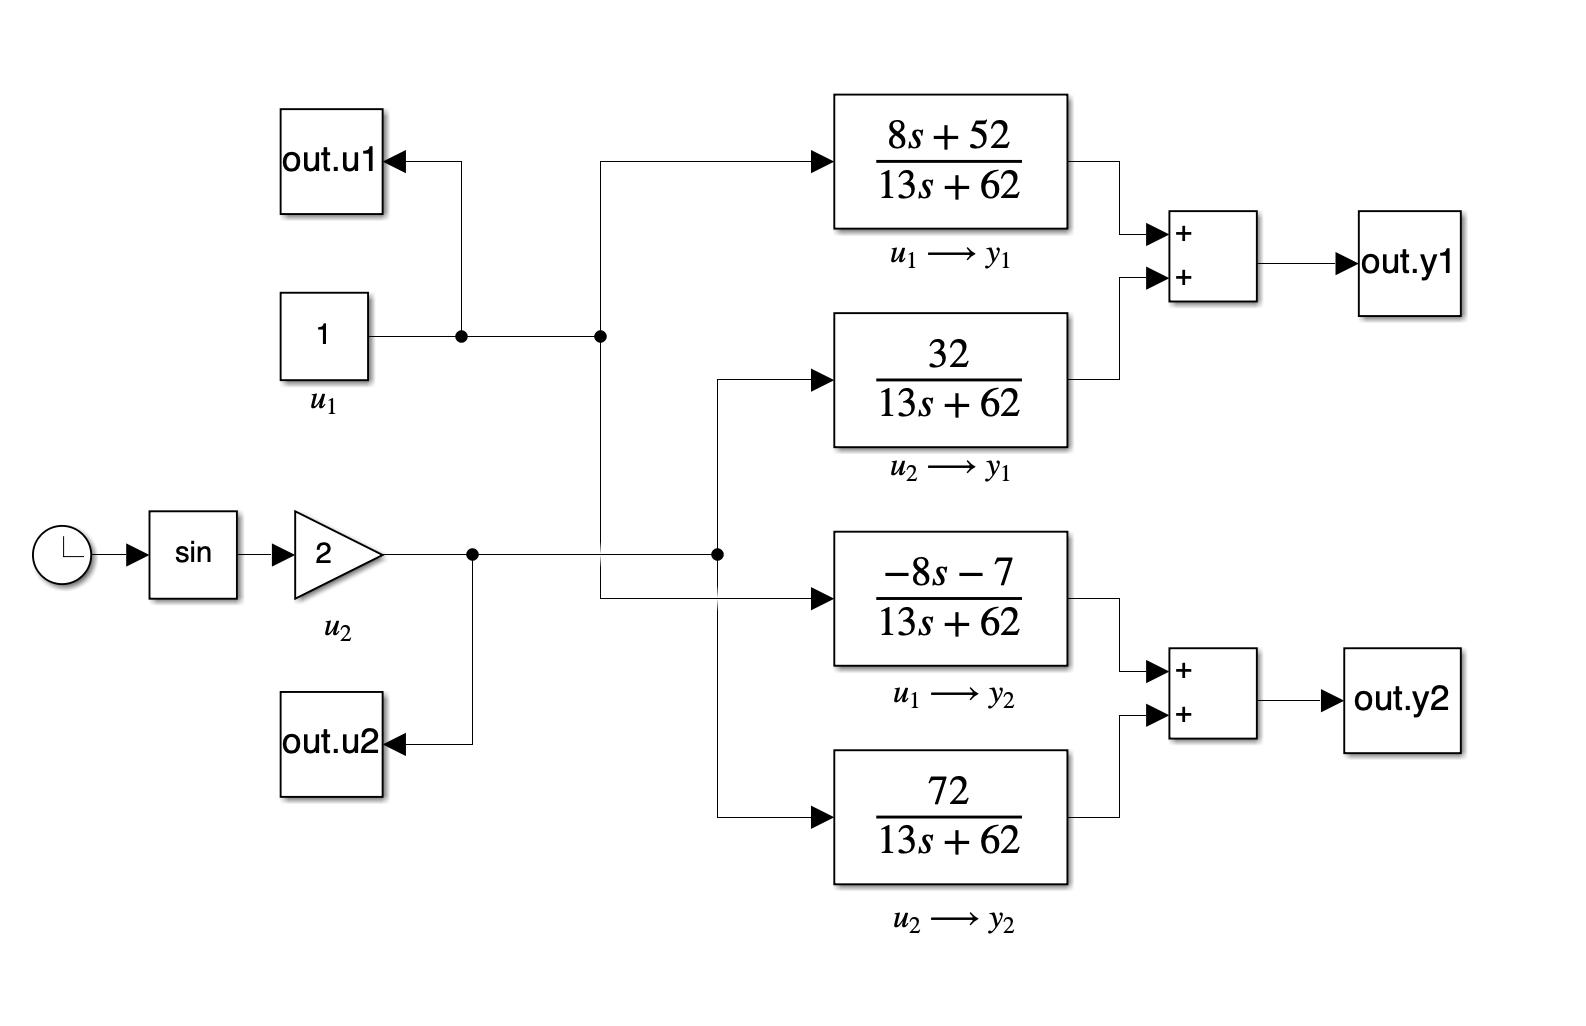
\includegraphics[width=0.8\textwidth]{media/system5.png}
    \caption{Схема многоканальной системы в форме вход-выход}
    \label{fig:MultyChannel}
\end{figure}

Промоделировав данную систему, получим графики $y_1(t)$ и $y_2(t)$, $u_1(t)$ и $u_2(t)$.

\begin{figure}[ht!]
    \centering
    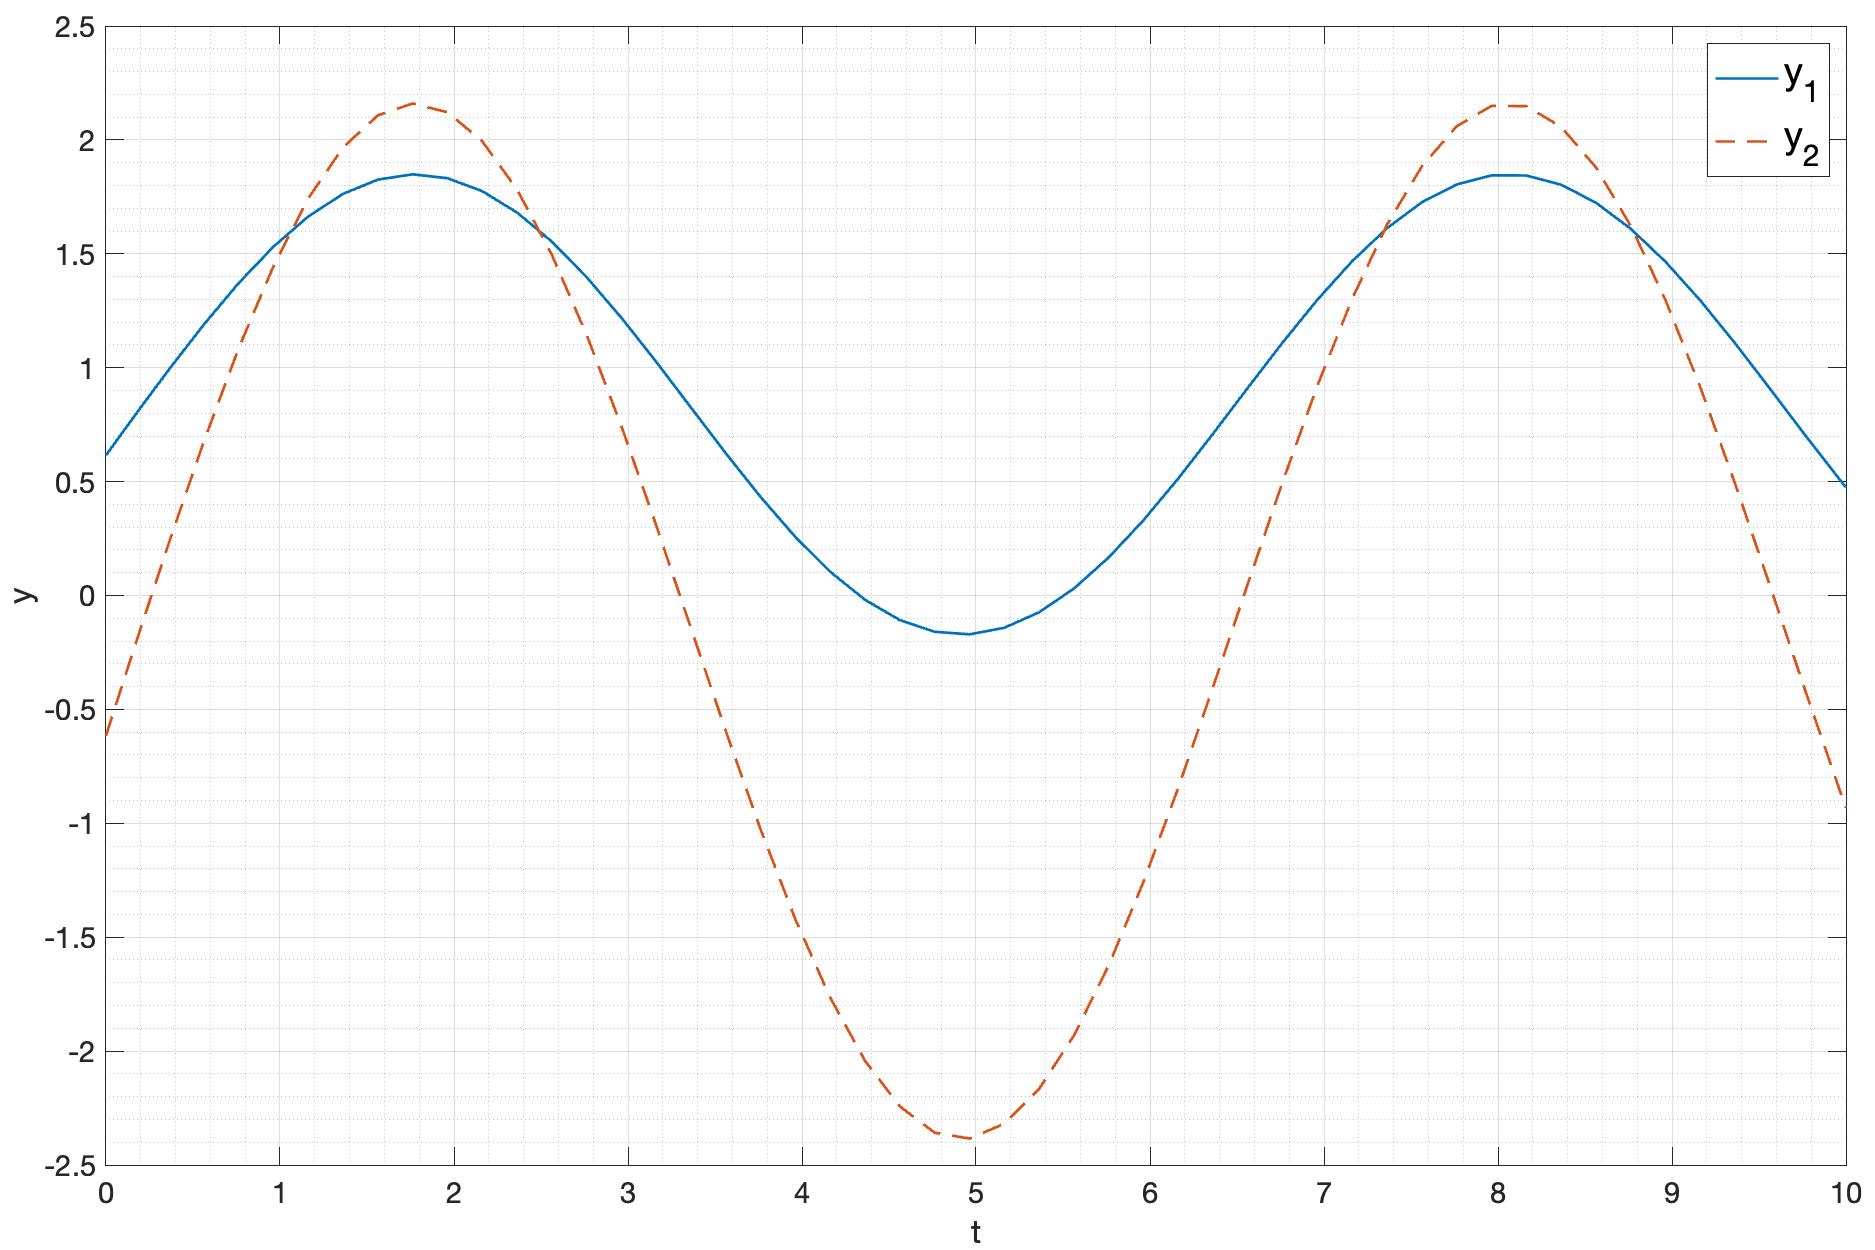
\includegraphics[width=\textwidth]{media/sys5_y(t).png}
    \caption{Графики $y_1(t)$ и $y_2(t)$}
    \label{fig:yt5}
\end{figure}

\begin{figure}[ht!]
    \centering
    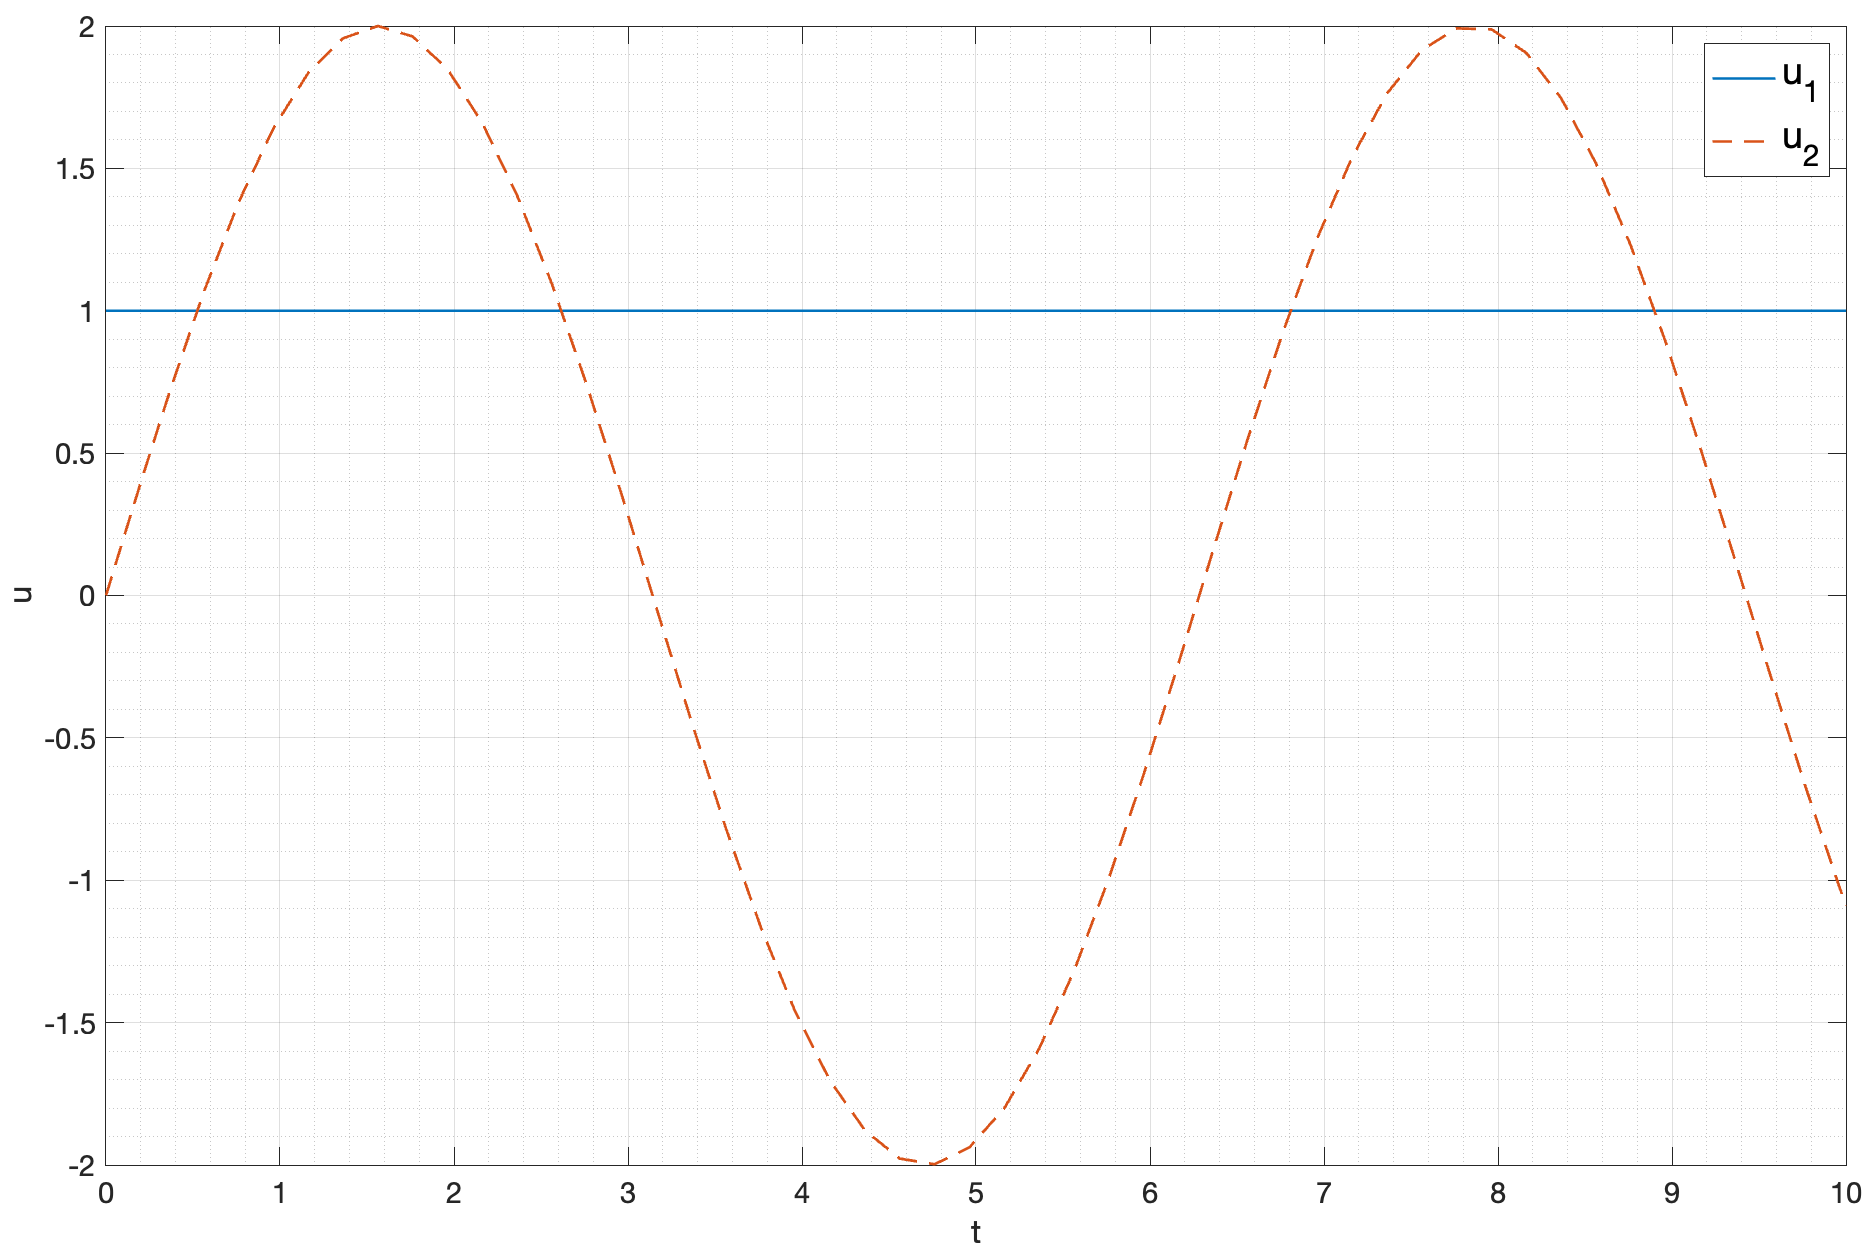
\includegraphics[width=\textwidth]{media/sys5_u(t).png}
    \caption{Графики $u_1(t)$ и $u_2(t)$}
    \label{fig:ut5}
\end{figure}

\FloatBarrier
\section{Многоканальная система в форме вход-состояние-выход}

Рассмотрим следующую систему:
\begin{equation}
    \begin{cases}
        \dot{x}(t) = A x + B u \\
        y(t) = Cx
    \end{cases}
\end{equation}

\begin{equation}
    A = \begin{bmatrix}
        0 & -9 \\
        1 & -3
    \end{bmatrix},~~~
    B = \begin{bmatrix}
        9 & 5 \\
        2 & 11
    \end{bmatrix},~~~
    C = \begin{bmatrix}
        5 & 6 \\
        3 & 8
    \end{bmatrix}
\end{equation}

Распишем систему в виде уравнений:
\begin{equation}
    \begin{cases}
        \dot{x}_1 = -9x_2 + -9u_1 + 5u_2 \\
        \dot{x}_2 = x_1 - 3x_2 + 2u_1 + 11u_2 \\
        y_1 = 5x_1 + 6x_2 \\
        y_2 = 3x_1 + 8x_2
    \end{cases}
\end{equation}

Теперь построим схему моделирования в Simulink.

\begin{figure}[ht!]
    \centering
    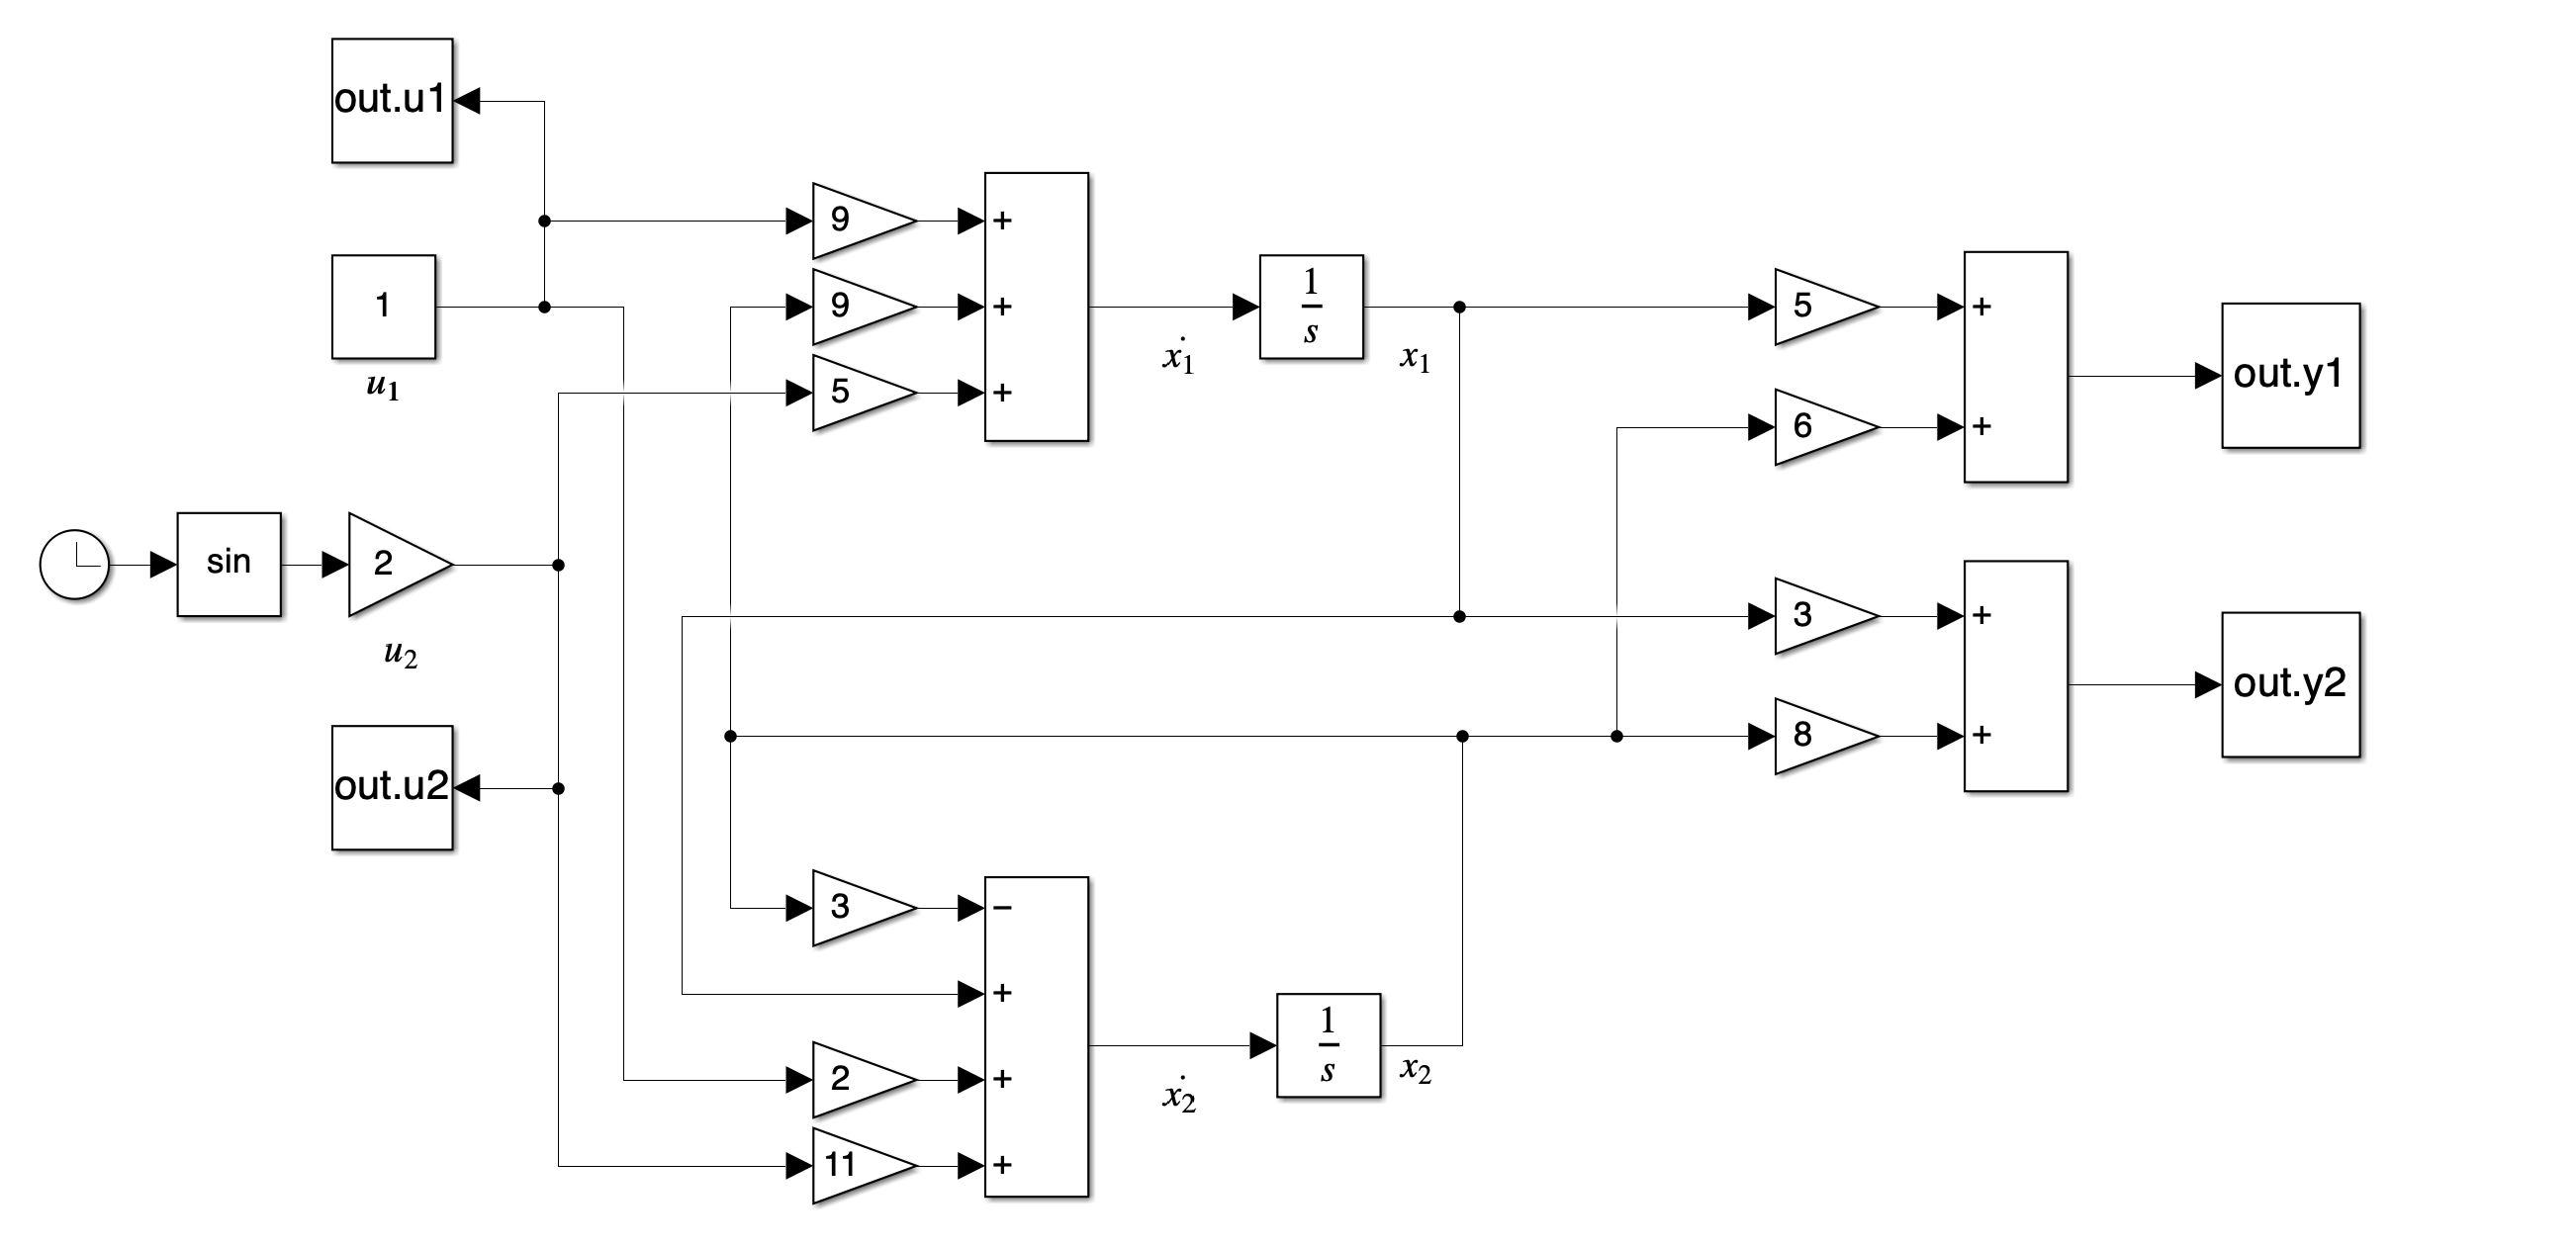
\includegraphics[width=0.8\textwidth]{media/system6.png}
    \caption{Схема многоканальной системы в форме вход-состояние-выход}
    \label{fig:model6}
\end{figure}

Промоделировав данную систему, получим графики $y_1(t)$ и $y_2(t)$, $u_1(t)$ и $u_2(t)$.

\begin{figure}[ht!]
    \centering
    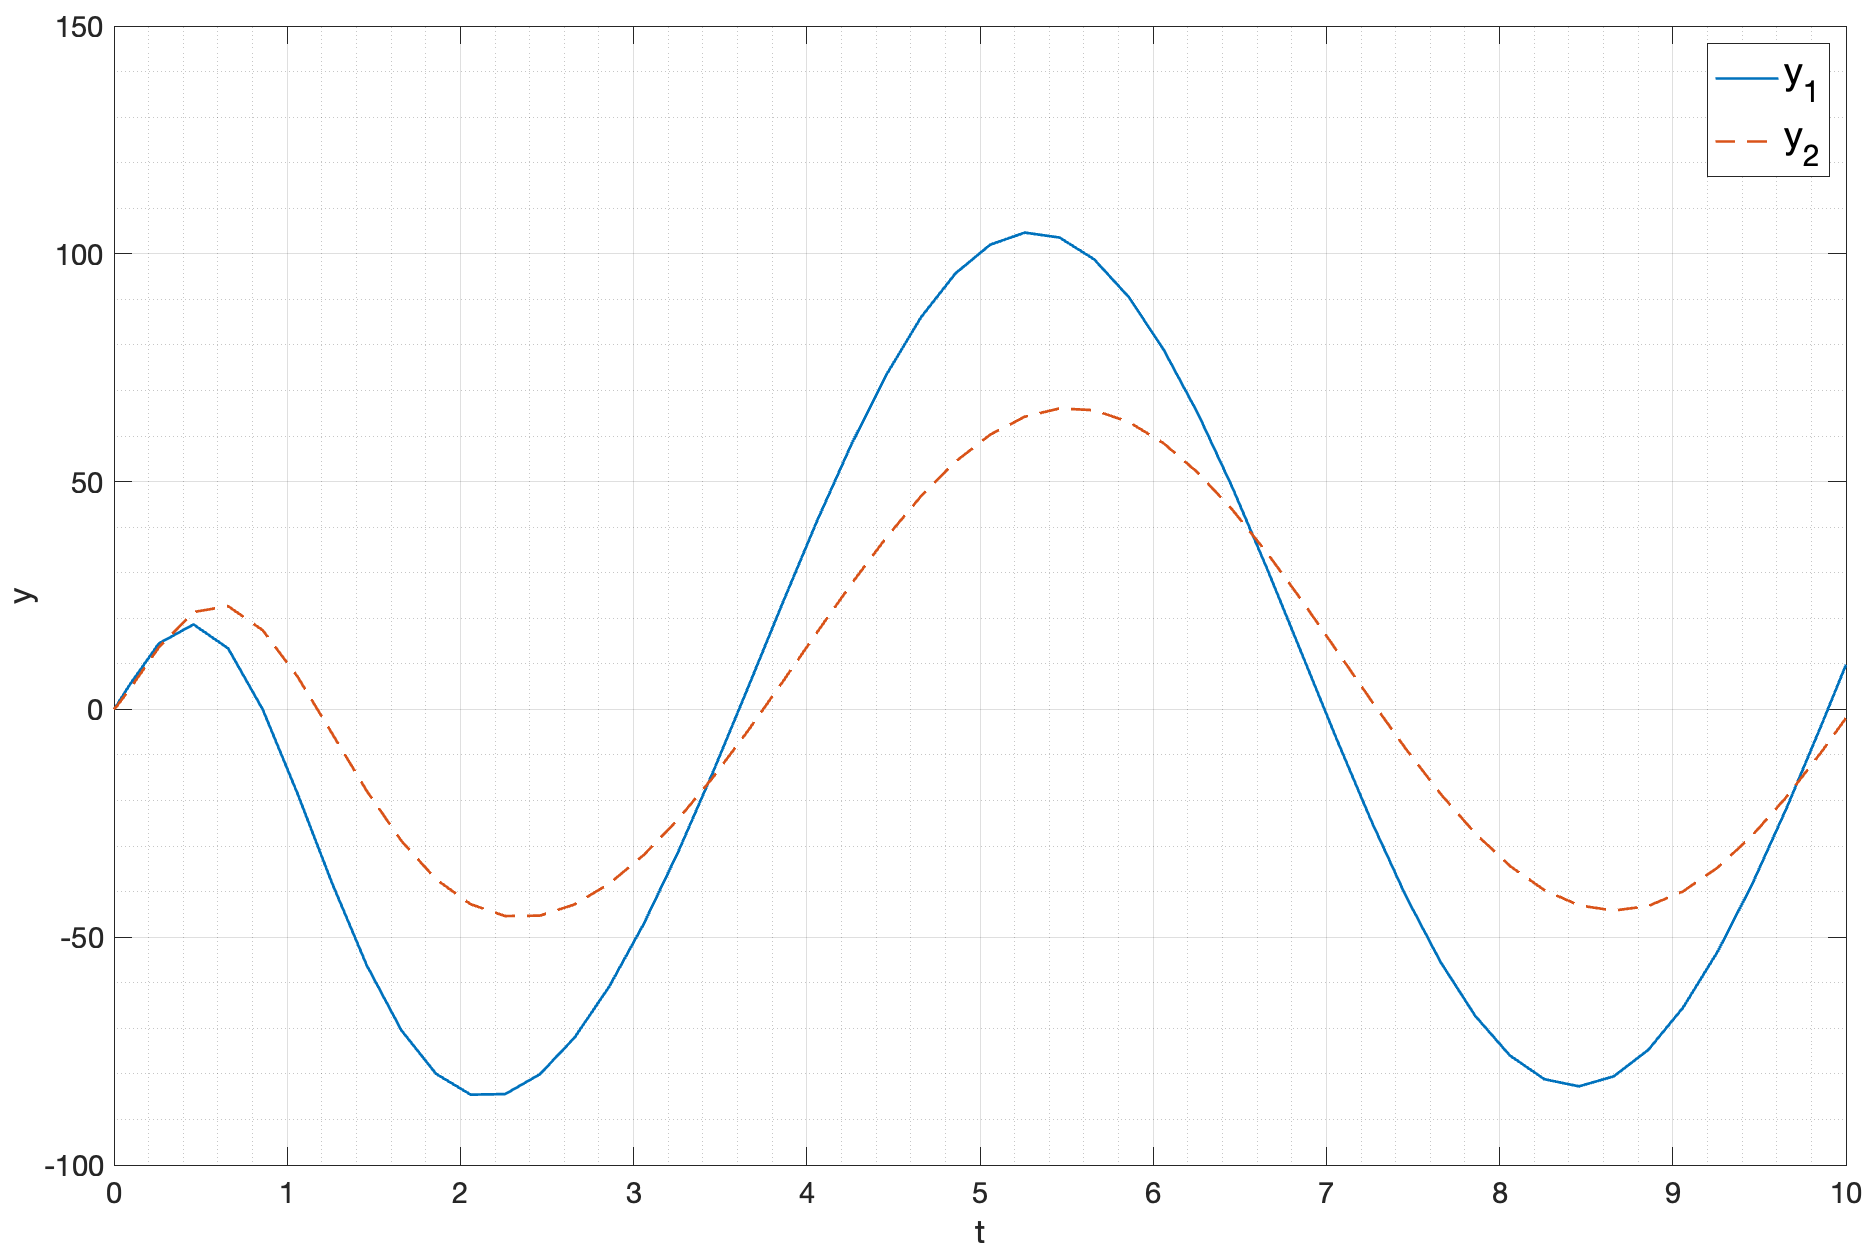
\includegraphics[width=\textwidth]{media/sys6_y(t).png}
    \caption{Графики $y_1(t)$ и $y_2(t)$}
    \label{fig:yt6}
\end{figure}

\begin{figure}[ht!]
    \centering
    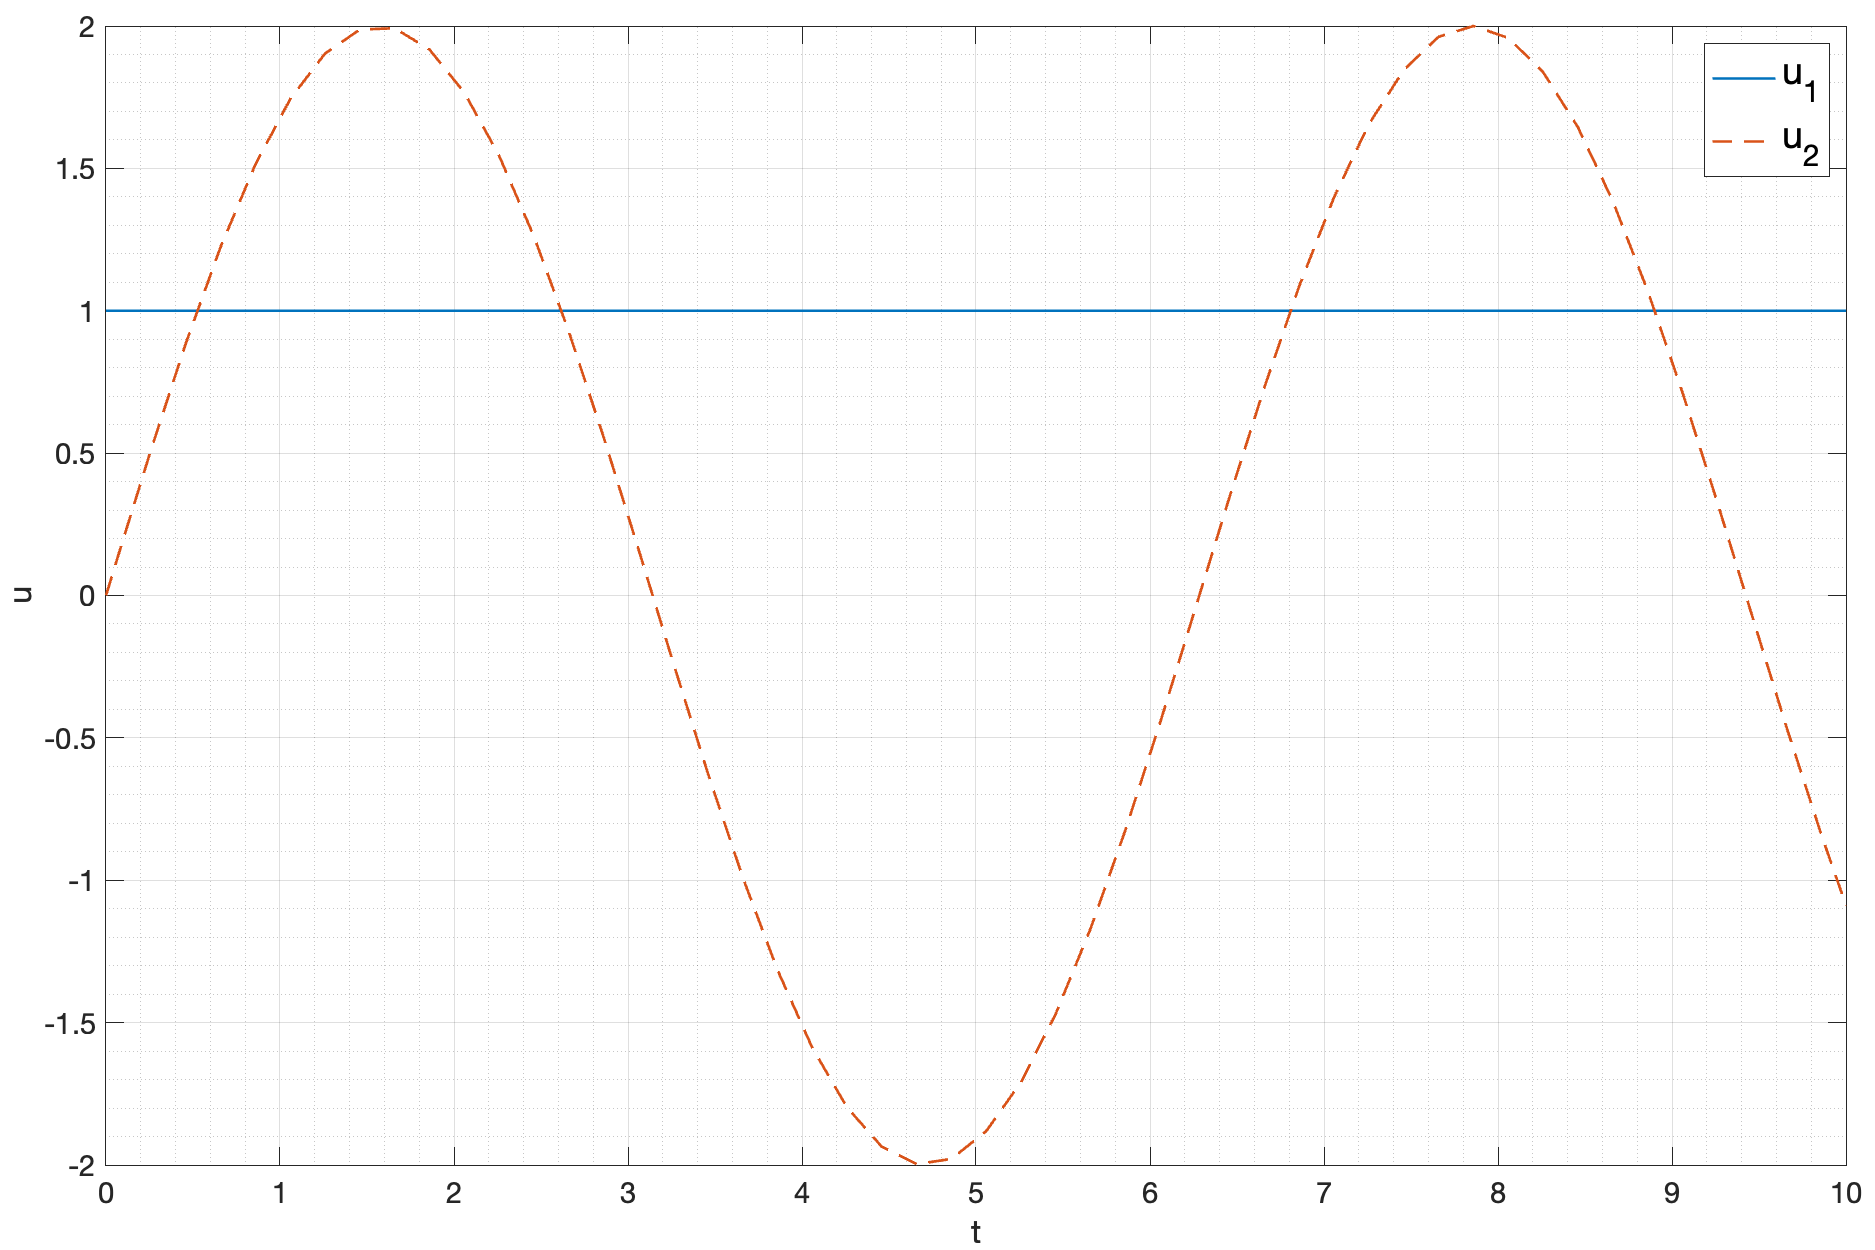
\includegraphics[width=\textwidth]{media/sys6_u(t).png}
    \caption{Графики $u_1(t)$ и $u_2(t)$}
    \label{fig:ut6}
\end{figure}